\section{Robot Design}
\label{sec:robot_design}

\subsection{The Single Vertical Manipulator Jump Model}

For a jumping robot, takeoff velocity determines jump height when air resistance is negligible. Consider a simple case of maximizing vertical jump height for a single-leg robot with a 2-DOF leg of equal link lengths.

The paw position relative to the body follows standard 2-link manipulator kinematics (equation \ref{eq:2_link_manipulator}, section \ref{sec:robot_kinematics}). For optimal vertical jumping, the body center of mass and paw move in opposite directions along the y-axis, as shown in figure \ref{fig:vertical_manipulator}. This constraint requires $\theta_1 = -\frac{(\theta_2+\pi)}{2}$ and $\dot{\theta}_2=-2\dot{\theta}_1$. Combining these with the end-effector Jacobian (equation \ref{eq:jacobian_vertical_jump_leg}), we can plot paw vertical velocity versus knee angle $\theta_2$ (figure \ref{fig:vertical_jacobian_velocity}), using equation \ref{eq:jacobian_speed_mapping}. 

Figure \ref{fig:vertical_jacobian_velocity} shows that joint velocity translates more effectively to body velocity when the knee is crouched. This indicates joint acceleration capability is as important as maximum speed when selecting motors - a faster motor provides little benefit unless it can also accelerate the joints more quickly.

\begin{figure}[h]
    \centering
    \includegraphics[width=0.75\textwidth]{Images/one_axis_jump.png}
    \caption{The manipulator corresponding to a vertical one leg jump.}
    \label{fig:vertical_manipulator}
\end{figure}

\begin{equation}
    \label{eq:2_link_manipulator}
    \begin{aligned}
        x_{\text{end}} &= L_1 \cos(\theta_1) + L_2 \cos(\theta_1 + \theta_2) \\
        y_{\text{end}} &= L_1 \sin(\theta_1) + L_2 \sin(\theta_1 + \theta_2)
    \end{aligned}
\end{equation}

\begin{equation}
    \label{eq:jacobian_vertical_jump_leg}
    J = \begin{bmatrix} 
    -L_1 \sin(\theta_1) - L_2 \sin(\theta_1 + \theta_2) & -L_2 \sin(\theta_1 + \theta_2) \\
    L_1 \cos(\theta_1) + L_2 \cos(\theta_1 + \theta_2) & L_2 \cos(\theta_1 + \theta_2)
    \end{bmatrix}
\end{equation}

\begin{figure}[h]
    \centering
    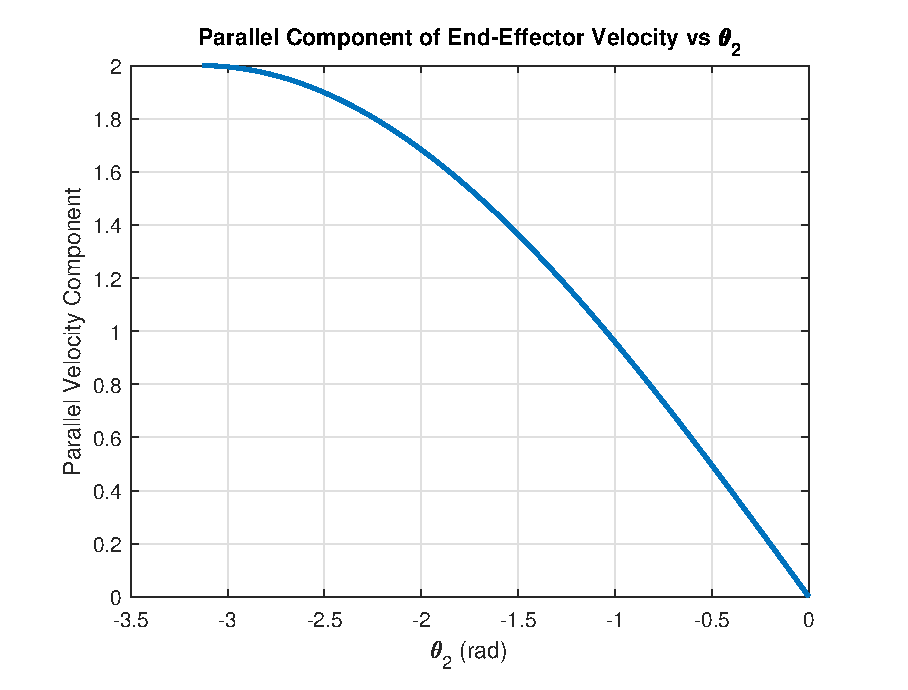
\includegraphics[width=\textwidth]{Images/vertical_paw_velocity.eps}
    \caption{Vertical Paw velocity as a function of knee angle.}
    \label{fig:vertical_jacobian_velocity}
\end{figure}

\subsection{Actuation Method Selection: Motors Only}
\label{sec:design_motor_only_jumps}

Initial experiments used motors alone. Motors from the supplier AGF-RC were selected for their high torque-to-weight ratio. The motor model used stall torque and maximum velocity parameters with linear torque decrease between them, as described in section \ref{sec:motor_modeling}. AGF-RC could not provide detailed performance data beyond these basic specifications. Motor-only actuation jumping performance was not satisfactory, thus the approach was abandoned. 

The A80BHP-H motor from AGF-RC had the highest stall torque and operating speed in its weight class. No comparable alternatives were found, making tests with this motor an optimistic baseline. Details are in appendix \ref{appendix:A80_motor_info}.

Tests applied maximum torque to knee motors in adherence with their torque-speed curve, while hip joints followed a control law (equation \ref{eq:friction_cone_limit}) to prevent slipping. This control law uses the force-torque mapping from section \ref{sec:force_torque_mapping} and friction theory from section \ref{sec:contact_friction}. Though equation \ref{eq:force_torque_mapping} assumes the system is in equilibrium, which is not valid for this dynamic jumping scenario, minimal slipping occurred in practice.

\begin{align}
    N &= \text{Normal force} \\
    \mu &= \text{friction coefficient} = 0.8 \\
    \tau_{\text{friction cone limit}} &= J^T 
    \begin{bmatrix}
        N \mu \\
        0
    \end{bmatrix} \\
    \max(|\tau_{knee}|) &= \tau_{\text{friction cone limit}}
    \label{eq:friction_cone_limit}
\end{align}

No leg configuration achieved satisfactory jumping height (defined as center of mass clearing ground by twice leg length). Results are detailed in section \ref{sec:results_motor_only_jumps}.

Later spring-motor experiments used weaker motors than the A80BHP-H motor, as well as more realistic friction models. The A80BHP-H was not used for spring-motor experiments because the motor supplier's website (see appendix \ref{appendix:A80_motor_info}) stated an operating travel limit of 90 degrees. Later contact with the supplier has revealed this to be false, and the operating travel limit for the A80BHP-H is in fact 180 degrees. For this reason, potential future use of the A80BHP-H motor with springs is discussed in section \ref{sec:future_work}.


\subsection{Actuation Method Selection: Motors and Extension Spring}

The extension spring design (figure \ref{fig:extension_spring_CAD}) was abandoned due to geometric constraints detailed in section \ref{sec:extension_spring_design}. Extension springs require attachment points at both ends, adding four design parameters that significantly affect jumping performance. The spring torque varies non-monotonically with knee angle $\theta_2$, and optimal attachment points depend heavily on link lengths. Including these parameters in the link length optimization (section \ref{sec:link_length_optimization}) would substantially increase complexity. 


\subsection{Actuation Method Selection: Motors and Torsional Spring}

The final design combines motors with torsional springs in the knees (figure \ref{fig:assembly_CAD}). Motors compress the knee springs until reaching a target angle. When released, the springs accelerate the joints for takeoff. Despite springs working against the friction of the motors as modelled in \ref{sec:motor_friction_estimation}, this achieved better jumping performance than motors alone, as shown in section \ref{sec:results:link_length_optimization}. 

In contrast to extension springs, since the spring force from a torsional spring depends only on its angular depelacement, it provides maximum torque at full knee flexion, most efficiently converting angular velocity into linear velocity at the paws.


\subsection{Hip Motor Strength Requirements}
\label{sec:hip_motor_dimensioning_test_design}

Successful jumping inherently requires aerial attitude stabilization for proper landing. The use of torsional knee springs for jumping reduces the hip motors' role in takeoff, allowing them to be optimized for aerial control. To validate that the hip motors can provide sufficient control authority for landing orientation, we adopted the heuristic from \cite{finn_tarek_master} of executing three 90-degree lateral swings per second. This benchmark provides a conservative bound on the torque and speed requirements needed to reorient the robot during flight.

We simulated this benchmark in Simulink Simscape, with the robot body fixed in space and 1cm diameter iron spheres (32g) as paws. While lighter than the 80g paws in \cite{finn_tarek_master}, this scales appropriately with our 300g body mass compared to their 800g. The simulation results are presented in section \ref{sec:hip_motor_dimensioning_test}.